%% LaTeX Beamer presentation template (requires beamer package)
%% see http://latex-beamer.sourceforge.net/
%% idea contributed by H. Turgut Uyar
%% template based on a template by Till Tantau
%% this template is still evolving - it might differ in future releases!

\documentclass[xcolor=svgnames]{beamer} 

% \mode<presentation>
% {
% \usetheme{Warsaw}
% 
% \setbeamercovered{transparent}
% }

\usetheme{Singapore}
\usepackage[english]{babel}
\usepackage[latin1]{inputenc}

% font definitions, try \usepackage{ae} instead of the following
% three lines if you don't like this look
\usepackage{mathptmx}
\usepackage[scaled=.90]{helvet}
\usepackage{courier} 


\usepackage[T1]{fontenc}

\usepackage{graphicx}
\usepackage{listings}
\usepackage{multirow}

%\hypersetup{colorlinks=true,linkcolor=red}

\def\hilite<#1>{%
\temporal<#1>{\color{gray}}{\color{black}}%
{\color{gray}}}
 
\title{Scenario Variability as Crosscutting Mechanisms}



% - Use the \inst{?} command only if the authors have different
%   affiliation.
%\author{F.~Author\inst{1} \and S.~Another\inst{2}}
\author{Rodrigo Bonif\'{a}cio \and Paulo Borba}

% - Use the \inst command only if there are several affiliations.
% - Keep it simple, no one is interested in your street address.
\institute
{
	Informatics Center \\ Federal University of Pernambuco \\ Brazil
}

% \date{\date() / SPLC Doctoral Symposium}


% This is only inserted into the PDF information catalog. Can be left
% out.
%\subject{Talks}



% If you have a file called "university-logo-filename.xxx", where xxx
% is a graphic format that can be processed by latex or pdflatex,
% resp., then you can add a logo as follows:

% \pgfdeclareimage[height=0.5cm]{university-logo}{university-logo-filename}
% \logo{\pgfuseimage{university-logo}}




% If you wish to uncover everything in a step-wise fashion, uncomment
% the following command:

%\beamerdefaultoverlayspecification{<+->}

%include polycode.fmt
%include lhs2tex.sty

\begin{document}

\lstset{language=haskell}

\begin{frame}
\titlepage
\end{frame}

\section{Introduction}

% \begin{frame}
% \frametitle{Software Product Line (SPL)}
% 
% \begin{block}{Definition}
% \begin{itemize}
%   \item The SPL approach is a well known technique for implementing systematic
%   reuse in software engineering.
%   \item Based on this approach, products are customized (or generated) from a
%   set of reusable assets.
% \end{itemize}
% \end{block}
% \end{frame}
 
 \begin{frame}
 \frametitle{Thesis Context}
 
\begin{block}{Software Product Line (SPLs)}
 \begin{itemize}
\item Systematic approach for software reuse
\item Products are customized from a set of reusable assets
\end{itemize}
 \center{
  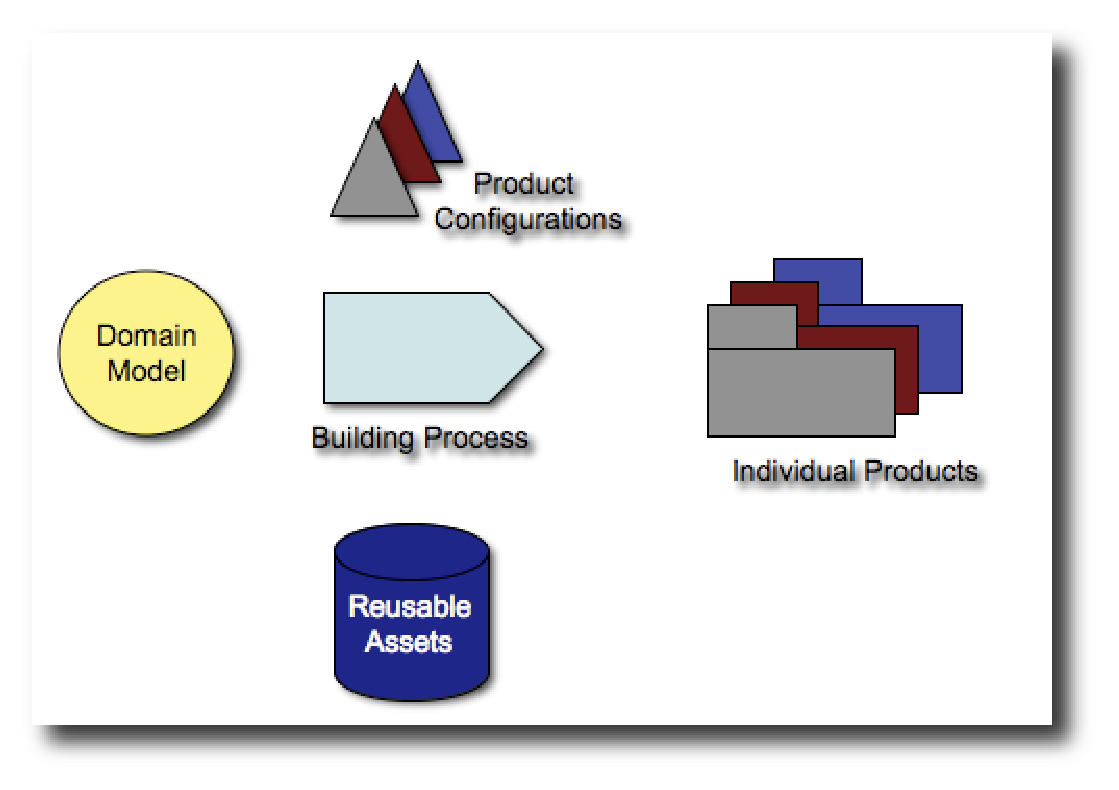
\includegraphics[scale=0.30]{img/spl.eps}
  }
\end{block}
 
 \end{frame}

\begin{frame}
\frametitle{Thesis Context}

\begin{block}{Crosscutting nature of variability management}
\begin{itemize}
	\item Variable features often require variation points to be scattered
	throughout different places in requirements, design, code, and test artifacts.
\end{itemize}
\end{block}

\onslide+<2>
\begin{block}{Consequence}
\begin{itemize}
   \item It is hard to evolve a SPL without a clear
  separation between the problem space, configuration space, and the solution space.
   \item Nevertheless, several techniques for dealing with
  variability present some kind of tangling between those models.    
\end{itemize}
\end{block}
\end{frame}


\begin{frame}
\frametitle{Motivating Example}
\begin{block}{SPL for Conference Management (CM-PL)}
\center{
  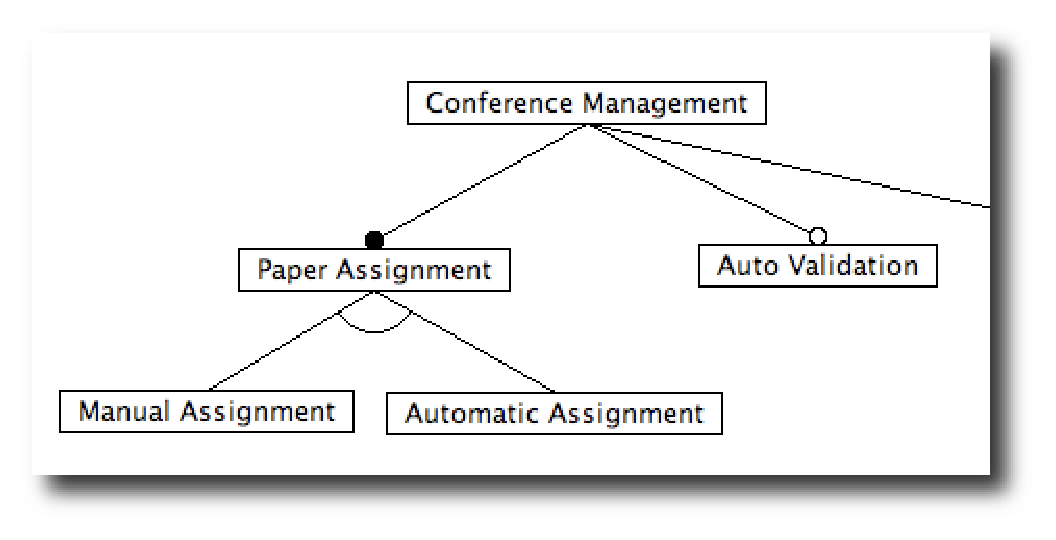
\includegraphics[scale=0.45]{img/cmtFinal01.eps}
  }
\end{block}
\end{frame}

\begin{frame}
\frametitle{Motivating Example}
\begin{block}{PLUSS specification of Paper Assignment}
\center{
  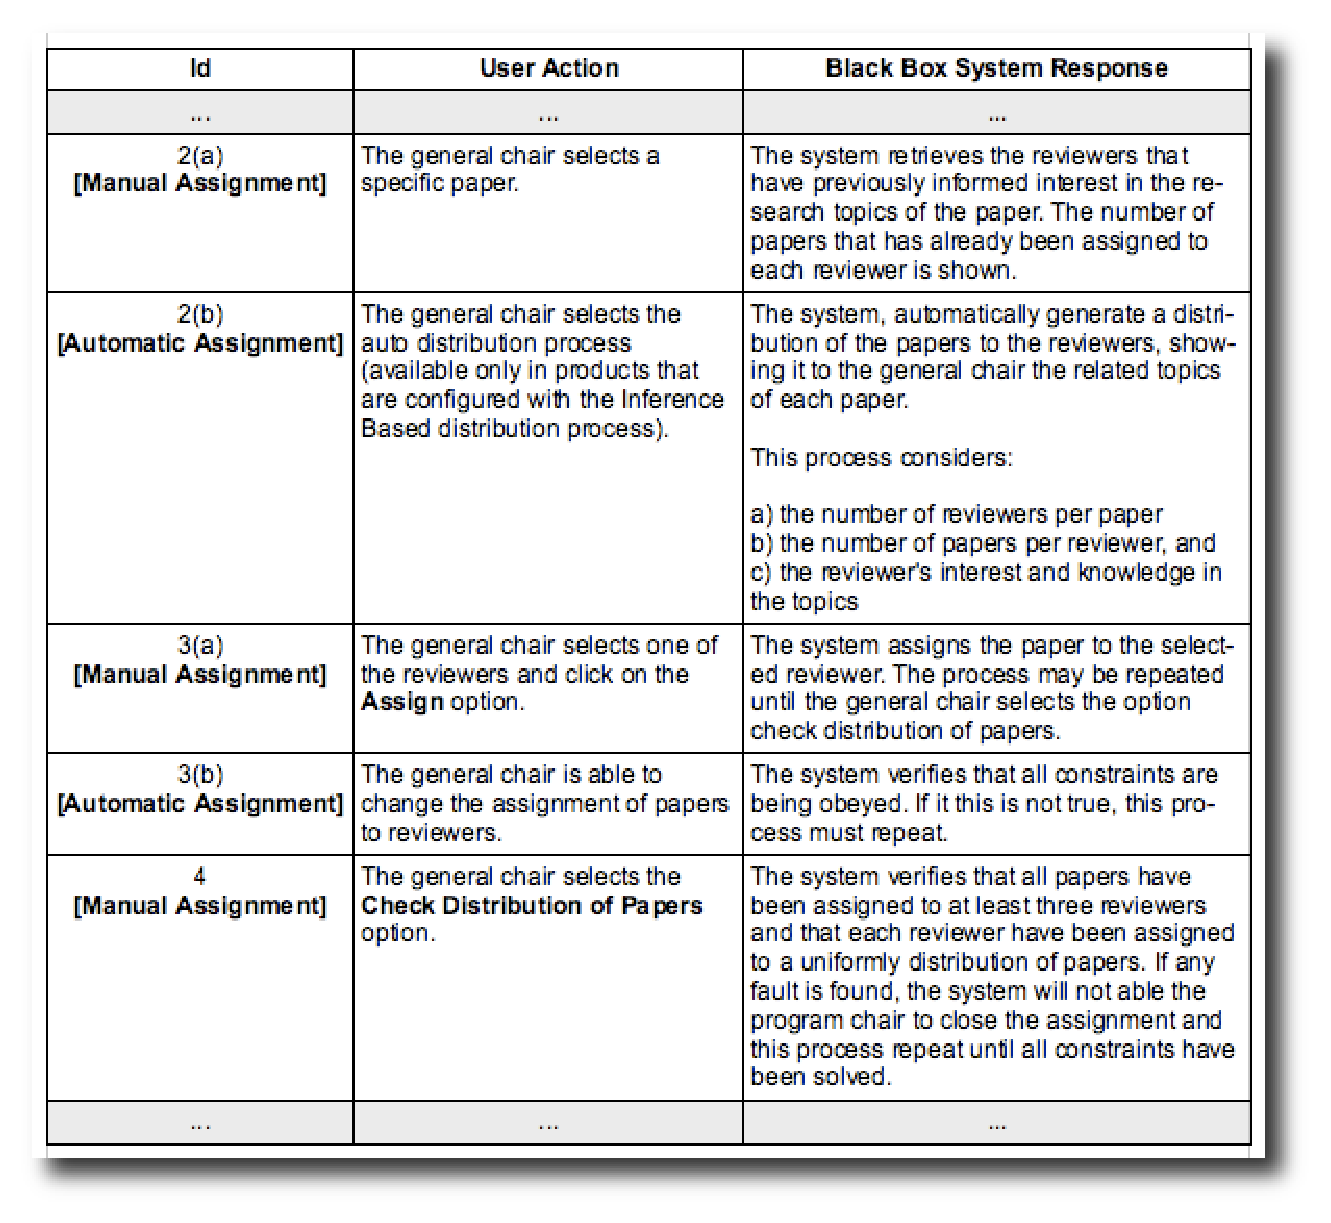
\includegraphics[scale=0.35]{img/pluss01.eps}
  }
 \end{block} 
\end{frame}

\begin{frame}
\frametitle{Motivating Example}
\begin{block}{PLUSS specification of Auto Validation}
\center{
  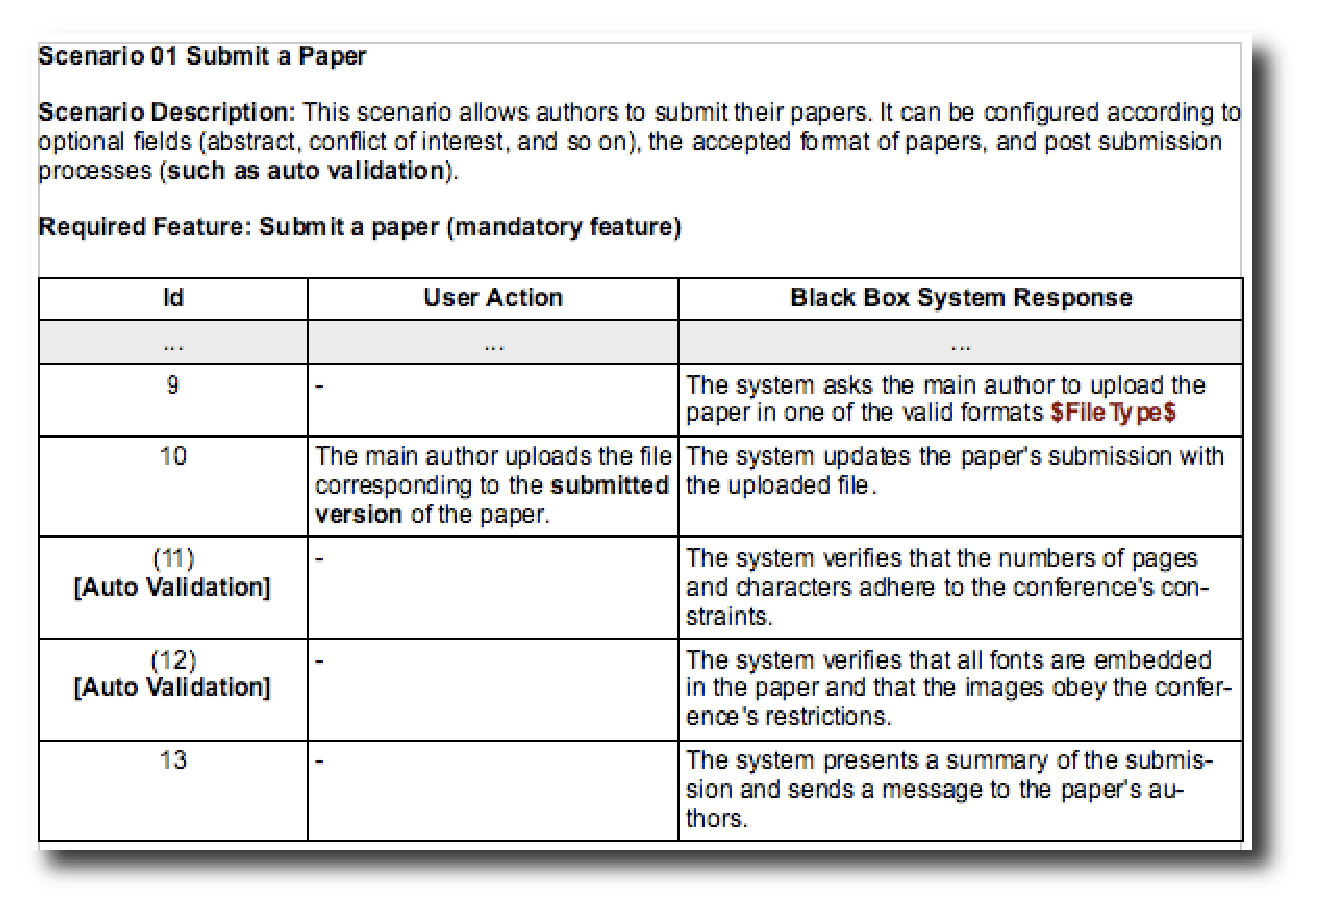
\includegraphics[scale=0.35]{img/pluss02.eps}
  }
\end{block}
\end{frame}

\begin{frame}
\frametitle{Motivating Example}
\begin{block}{PLUSS specification of Auto Validation}
\center{
  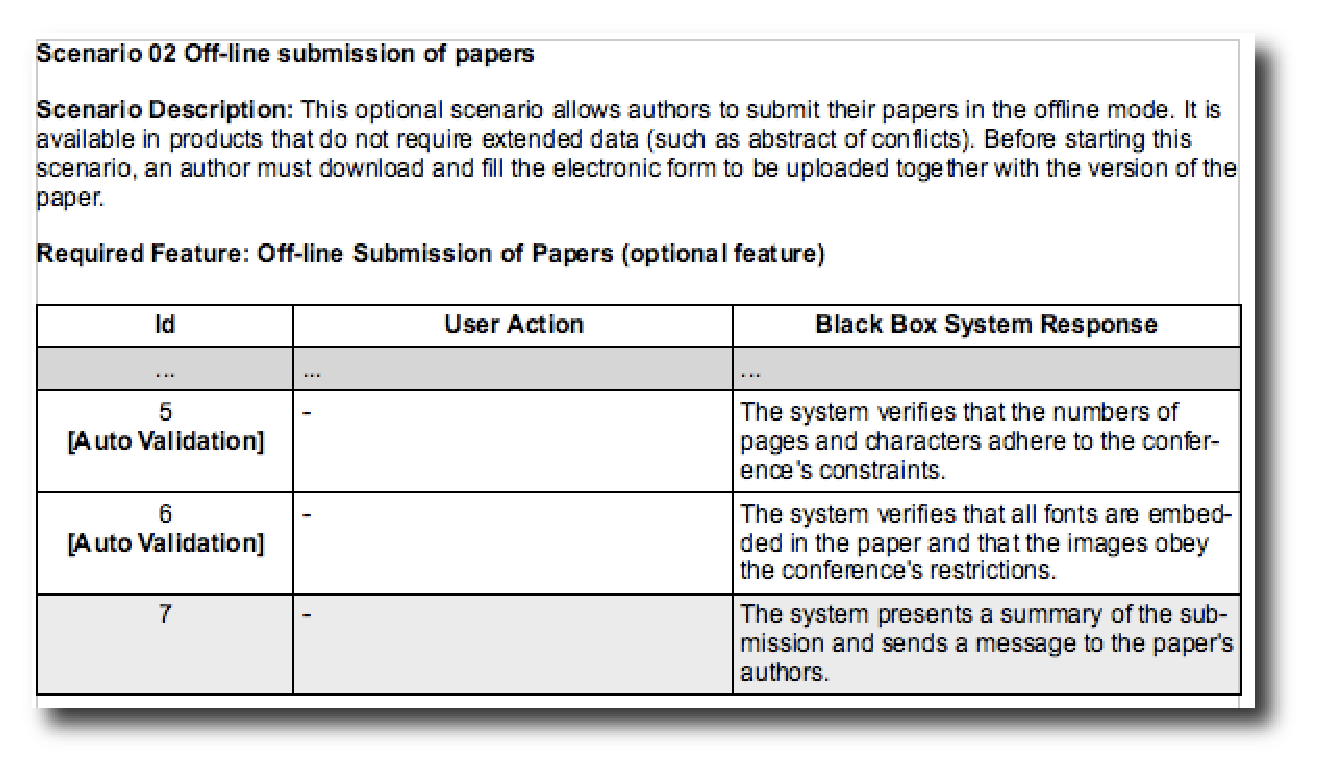
\includegraphics[scale=0.35]{img/pluss03.eps}
  }
 \end{block} 
\end{frame}

\begin{frame}
\frametitle{Motivating Example}
\begin{block}{SPL for Conference Management}
\center{
  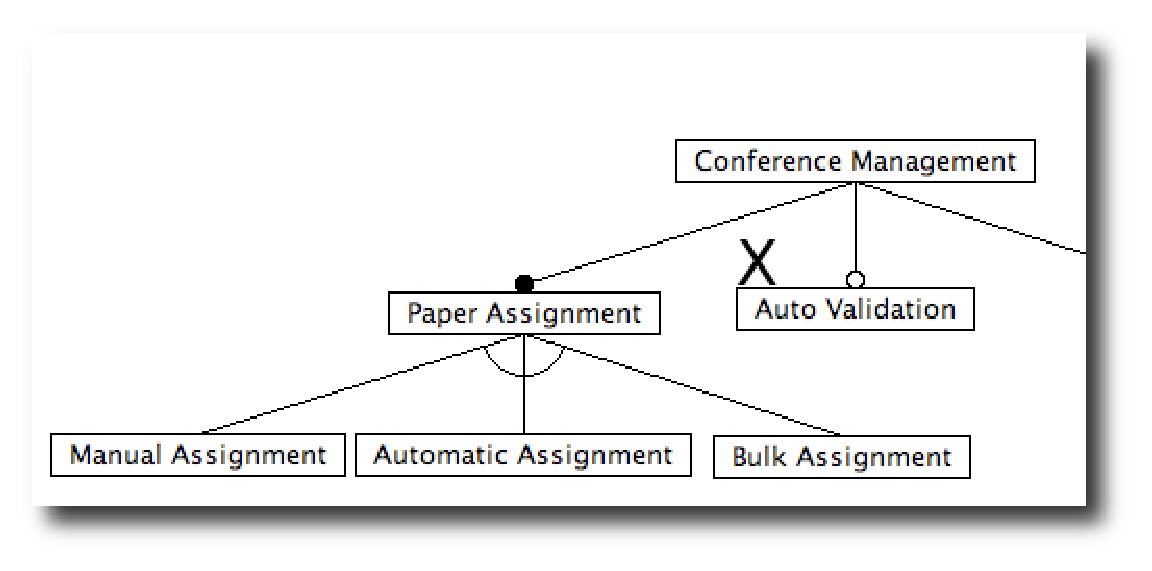
\includegraphics[scale=0.45]{img/cmtFinal02.eps}
  }
\end{block}
\end{frame}

\begin{frame}
\frametitle{Motivating Example}
\begin{block}{Resulting problems}
\begin{itemize}
\item Feature scattering (hard to maintain)
\item Scenarios present low level of cohesion (hard to understand)
\item Introducing new variants of a feature is painful
\end{itemize}
\end{block}
\end{frame}

\begin{frame}
\frametitle{Objective}

Improving the SoC between scenario specifications and variability management. 

\begin{block}{Relevance}
Use case scenarios are used as input for several activities, such as:
\begin{itemize}
\item SPL architecture and design
\item Test cases generation
\item Writing of the user manual 
\end{itemize}
\end{block}
\end{frame}

\begin{frame}
\frametitle{Proposed Solution}
A new approach for scenario variability management, which considers the 
following properties:

\begin{itemize}
  \item Support for different kinds of variation
  \item Better SoC between VM and scenarios specifications 
\end{itemize}

\onslide+<2>
\begin{block}{Notation}
A modeling framework for representing variability management techniques as
crosscutting mechanisms.
\begin{itemize}
  \item But we are not only talking about independent models for VM
  \item We also consider the \textcolor{DarkBlue}{composition processes}
  of these models
\end{itemize}
\end{block}
\end{frame}

\section{Proposed approach}

\begin{frame}
\frametitle{VM as Crosscutting Mechanisms}

During the product generation phase, different input models crosscut each other
with respect to a SPL member (adapted from Masuhara and Kiczales --- ECOOP 2003).

\onslide+<2>
\begin{block}{Big picture:}
\center{
 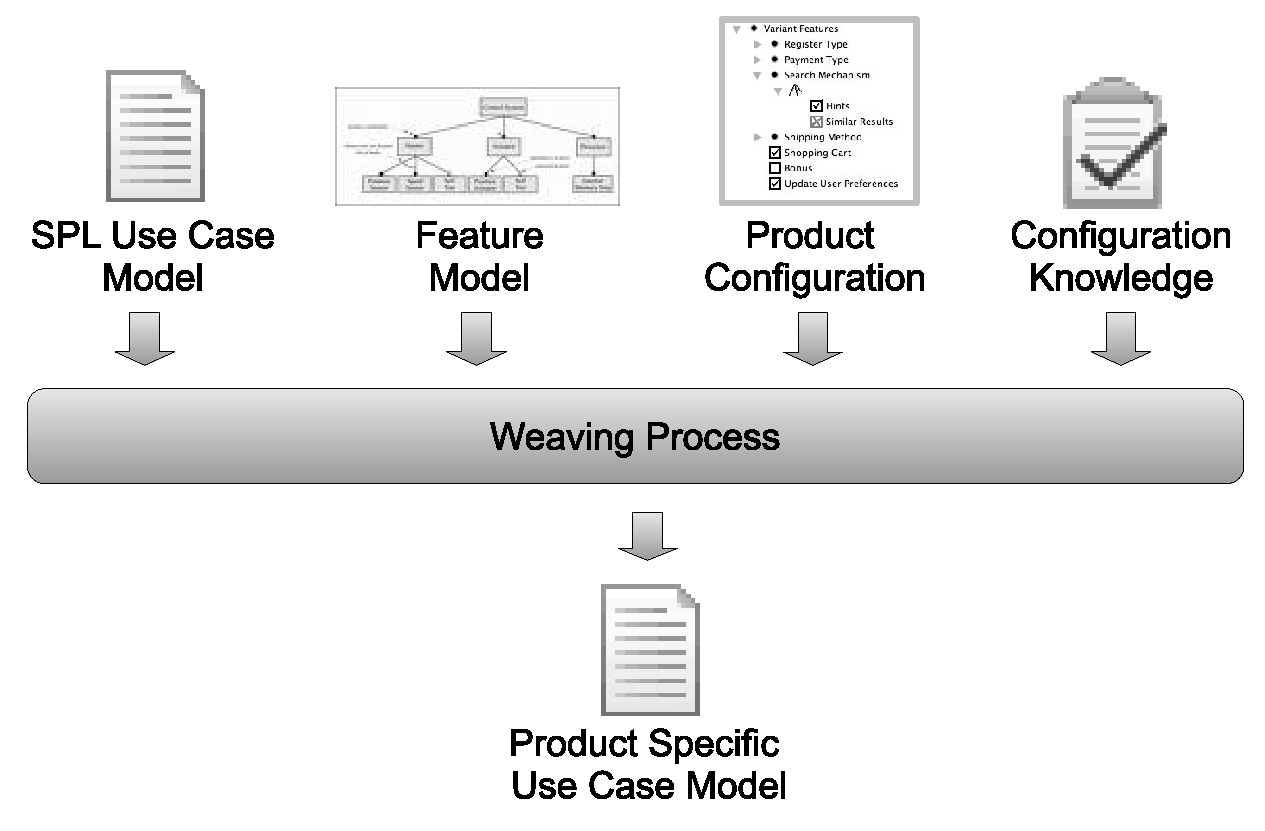
\includegraphics[scale=0.25]{img/weave-process2.eps}
}
\end{block}

\end{frame}

\begin{frame}
\frametitle{VM as Crosscutting Mechanisms}
\begin{block}{Weaving Processes}
\begin{itemize}
  \hilite<1> \item Sequence of transformations (weavers, tasks), guided by the
  configuration knowledge, which should be applied in order to generate specific instances.
  \hilite<2> \item Each weaver is represented as a
  tuple that highlights the contribution of the
  corresponding input languages. \\ 
  $Weaver = \{O,\ O_{VP},\ L,\ L(l)_{id},\
  	L(l)_{eff}\}$
\hilite<3> \item We depict that a weaver is
  	realizable by relating the corresponding tuple elements to a reference implementation of the weaver.
\end{itemize}	
\end{block}

\end{frame}

\begin{frame}
\frametitle{Configuration Knowledge}
\begin{center}
\begin{tabular}{||lp{1.4in}||}
\hline
Feature Expression  						& Tasks					 \\ \hline

\multirow{2}{*}{eShop}						& select scenario {\bf SC01} \\
										& select scenario {\bf SC02} \\	\hline
{\bf not} (Shopping Cart {\bf and} Bonus) 			& evaluate advice {\bf ADV01} \\
\hline (Shopping Cart {\bf and} Bonus) 			& evaluate advice {\bf ADV02} 	\\
\hline Update User Preferences 				& evaluate advice {\bf ADV03} \\ \hline
Shipping Method							& bind parameter {\bf SM}\\ \hline
								
\end{tabular}
\end{center}
\end{frame}

\begin{frame}
\frametitle{Configuration Knowledge}
\begin{center}
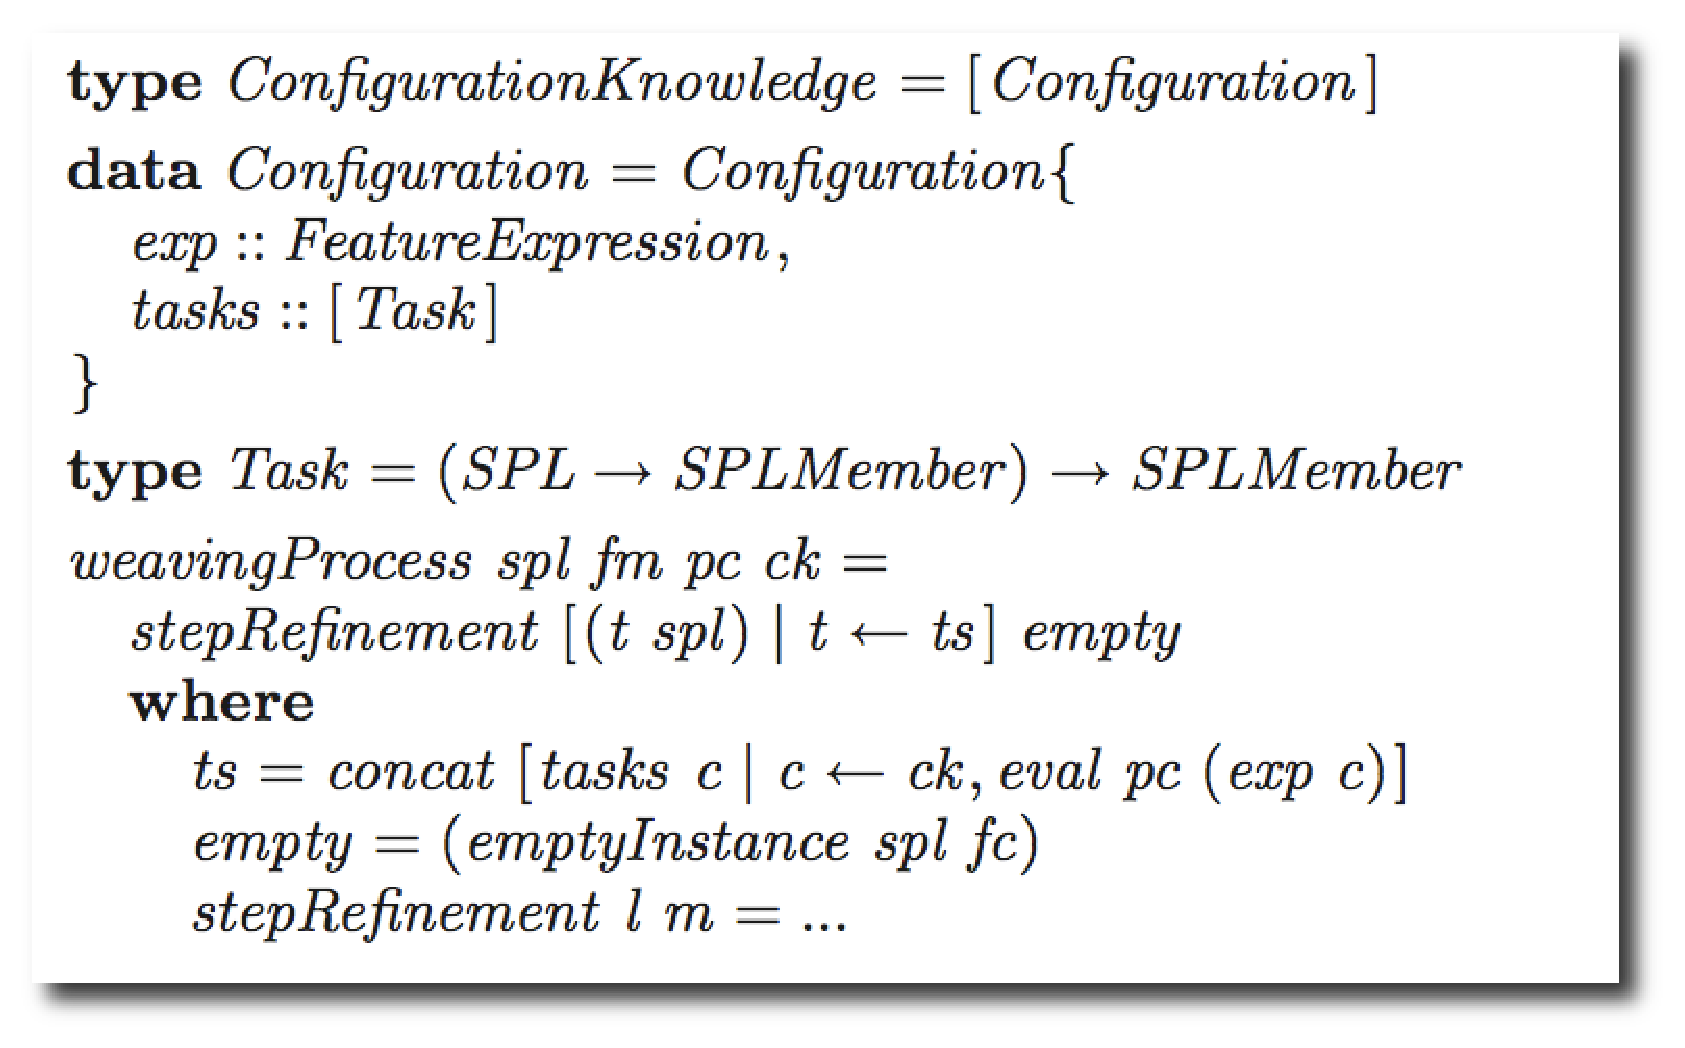
\includegraphics[scale=0.35]{img/ckFinal03.eps}
\end{center}
\end{frame}

\section{Modeling framework instance}

\begin{frame}
\frametitle{Kinds of Variability}
One instance of the modeling framework for each kind of variability.

\begin{itemize}
    \item Variability in function
    \item Variability in data
    \item Variability in control flow
\end{itemize}


\end{frame}

\begin{frame}
\frametitle{Variability in Function}
Certain use cases and scenarios of a SPL might exist in some
products and not in others.

\begin{block}{Examples}
\begin{scriptsize}
\begin{center}
\begin{tabular}{|p{1.6in}p{0.4in}p{1.6in}|}
\hline 
Artifact &  & Feature \\ \hline
\ldots & & \ldots \\ \hline
Assign Papers to Reviewers & requires & Paper Assignment \\ \hline
Off-line submission of papers & requires & Off-line Submission \\ \hline
Auto Conflict Detection & requires & Conflict Detection {\bf and} \ldots \\
\hline

\ldots & & \ldots \\
\hline
\end{tabular}
\end{center}
\end{scriptsize}
\end{block}

\end{frame}

\begin{frame}
\frametitle{Variability in Data}
Certain scenarios of a SPL might be parameterized.

\begin{block}{Example: different formats might be accepted (PS, PDF, DOC)}

\begin{center} 
\center{
 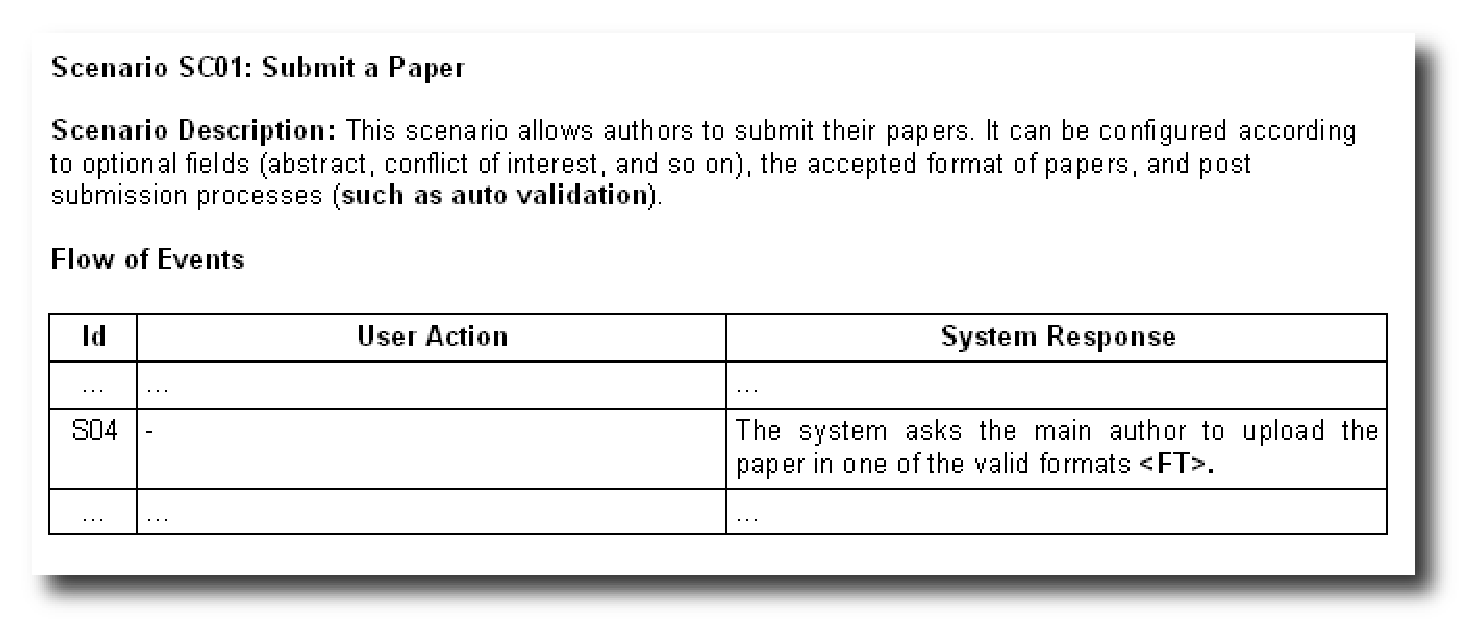
\includegraphics[scale=0.35]{img/scParameter.eps}
}

\end{center}
\end{block}
\end{frame}

\begin{frame}
\frametitle{Variability in Control Flow}
The flow of events of certain scenarios might vary.

\begin{block}{Example: Assign papers to reviewers}

\begin{center} 
\center{
 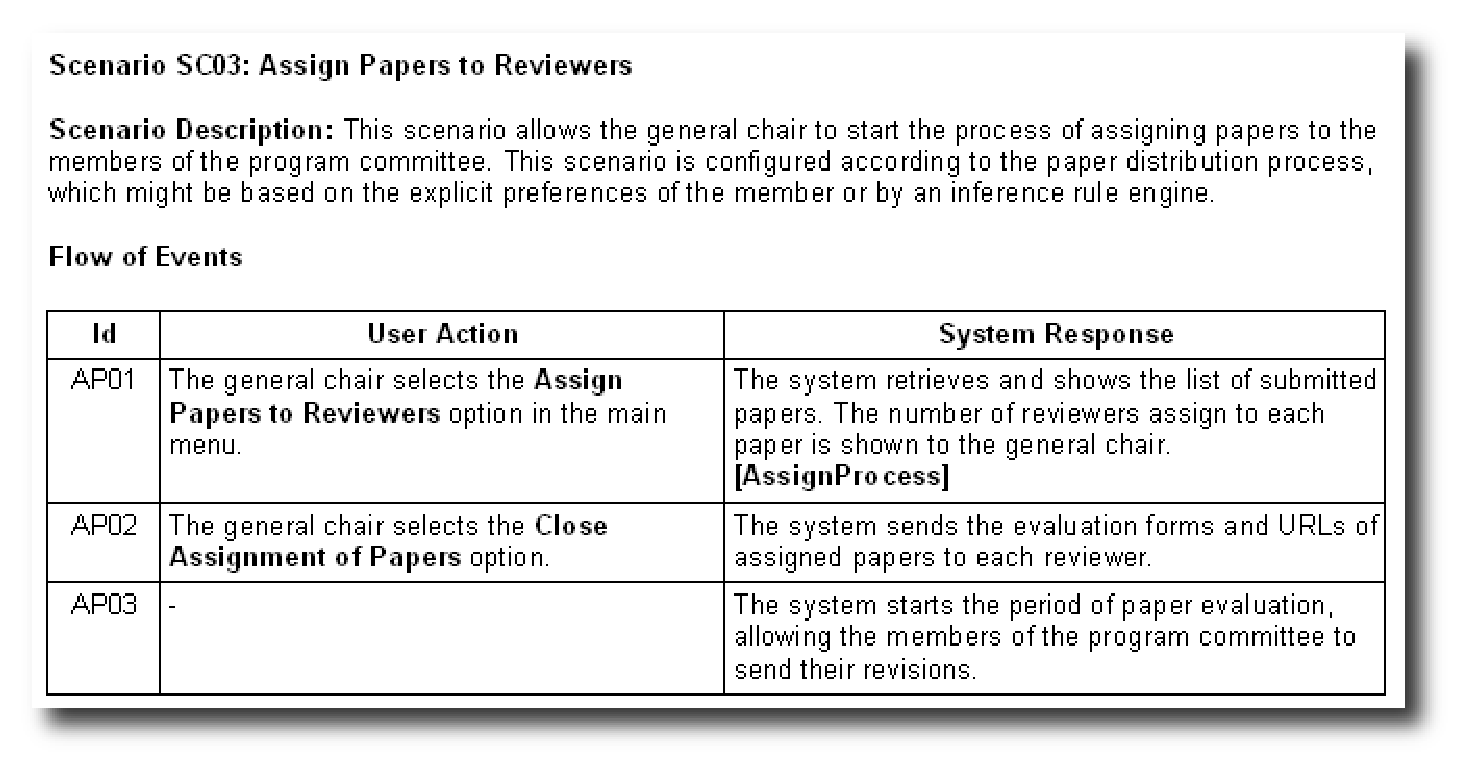
\includegraphics[scale=0.35]{img/scAssignPapers.eps}
}
\end{center}

\end{block}

\end{frame}

\begin{frame}
\frametitle{Variability in Control Flow}

\begin{block}{Manual Assignment}
\begin{center} 
\center{
 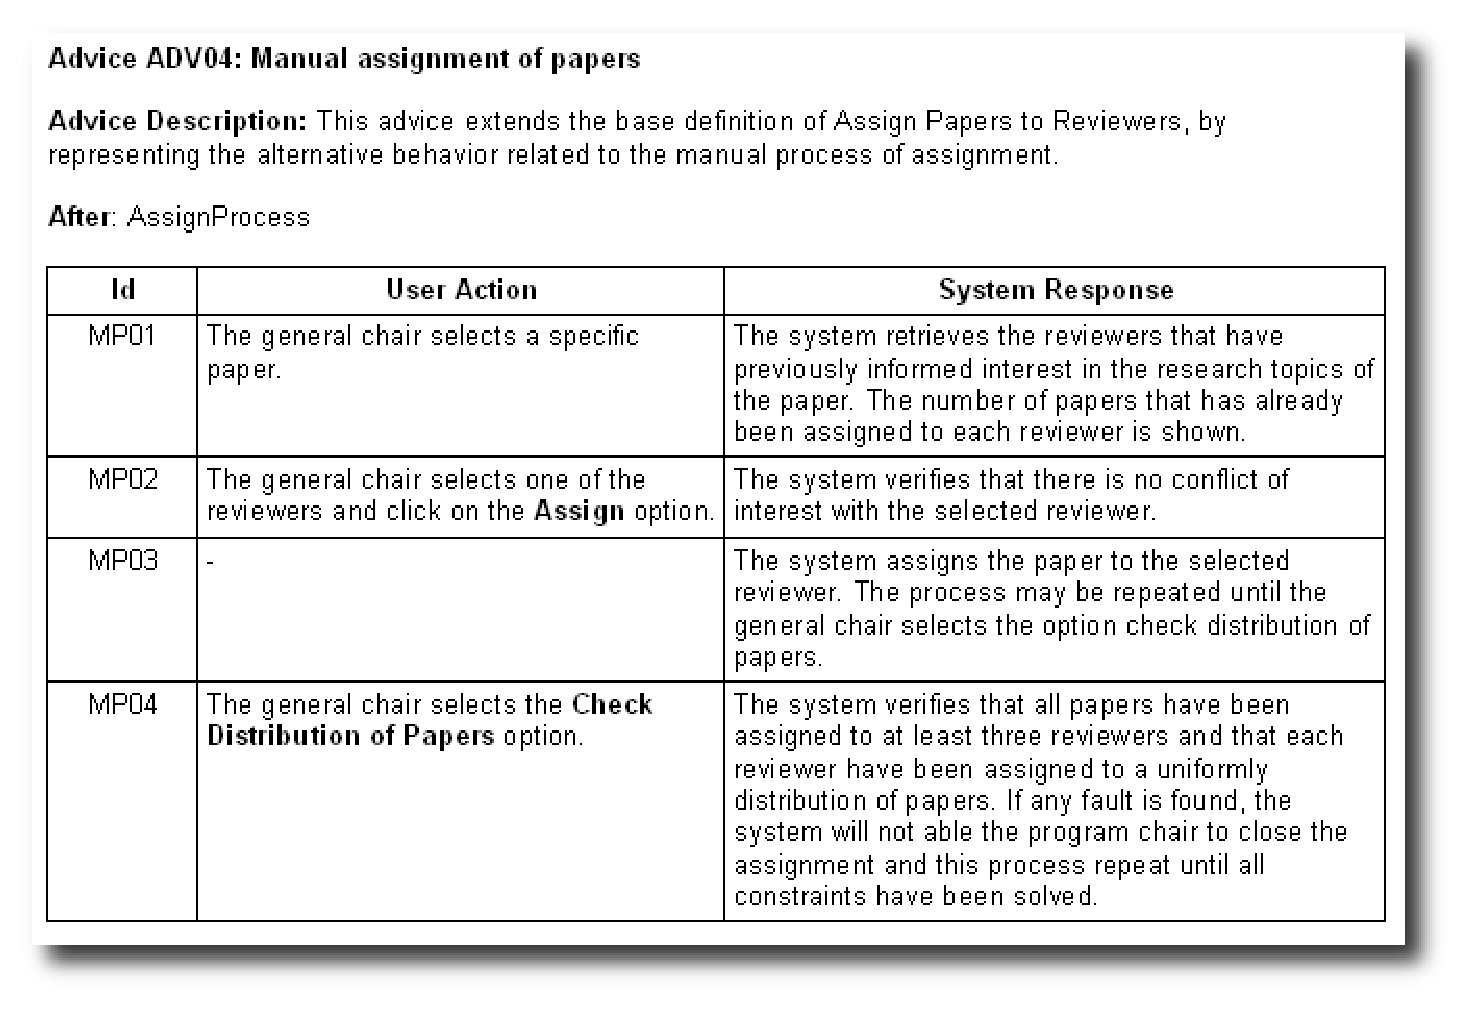
\includegraphics[scale=0.35]{img/advManualAssignment.eps}
}
\end{center}
\end{block}
\end{frame}

\begin{frame}
\frametitle{Variability in Control Flow}

\begin{block}{Automatic Assignment}
\begin{center} 
\center{
 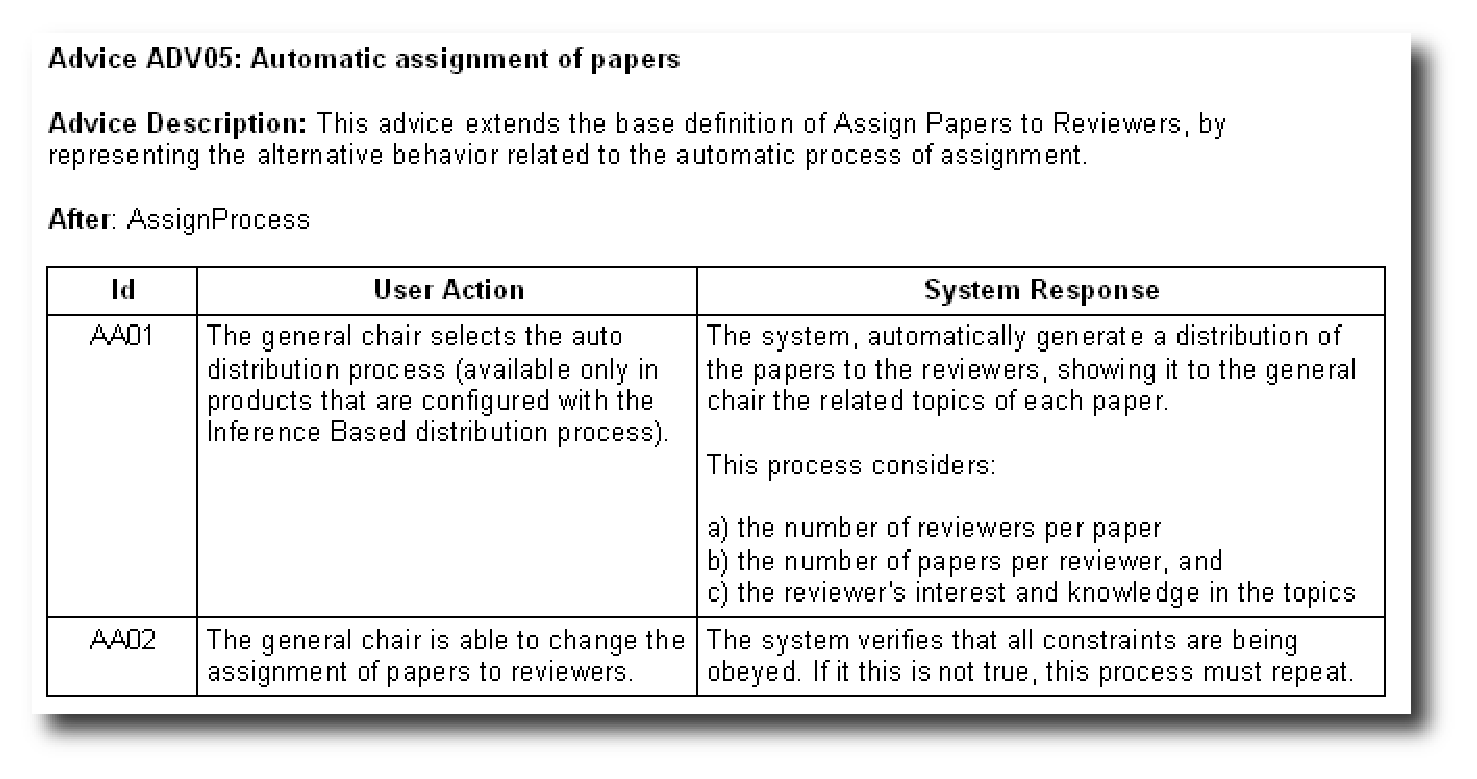
\includegraphics[scale=0.35]{img/advAutomaticAssignment.eps}
}
\end{center}
\end{block}
\end{frame}

\begin{frame}
\frametitle{Variability in Control Flow}
\begin{block}{Reference implementation}
\begin{center} 
\center{
 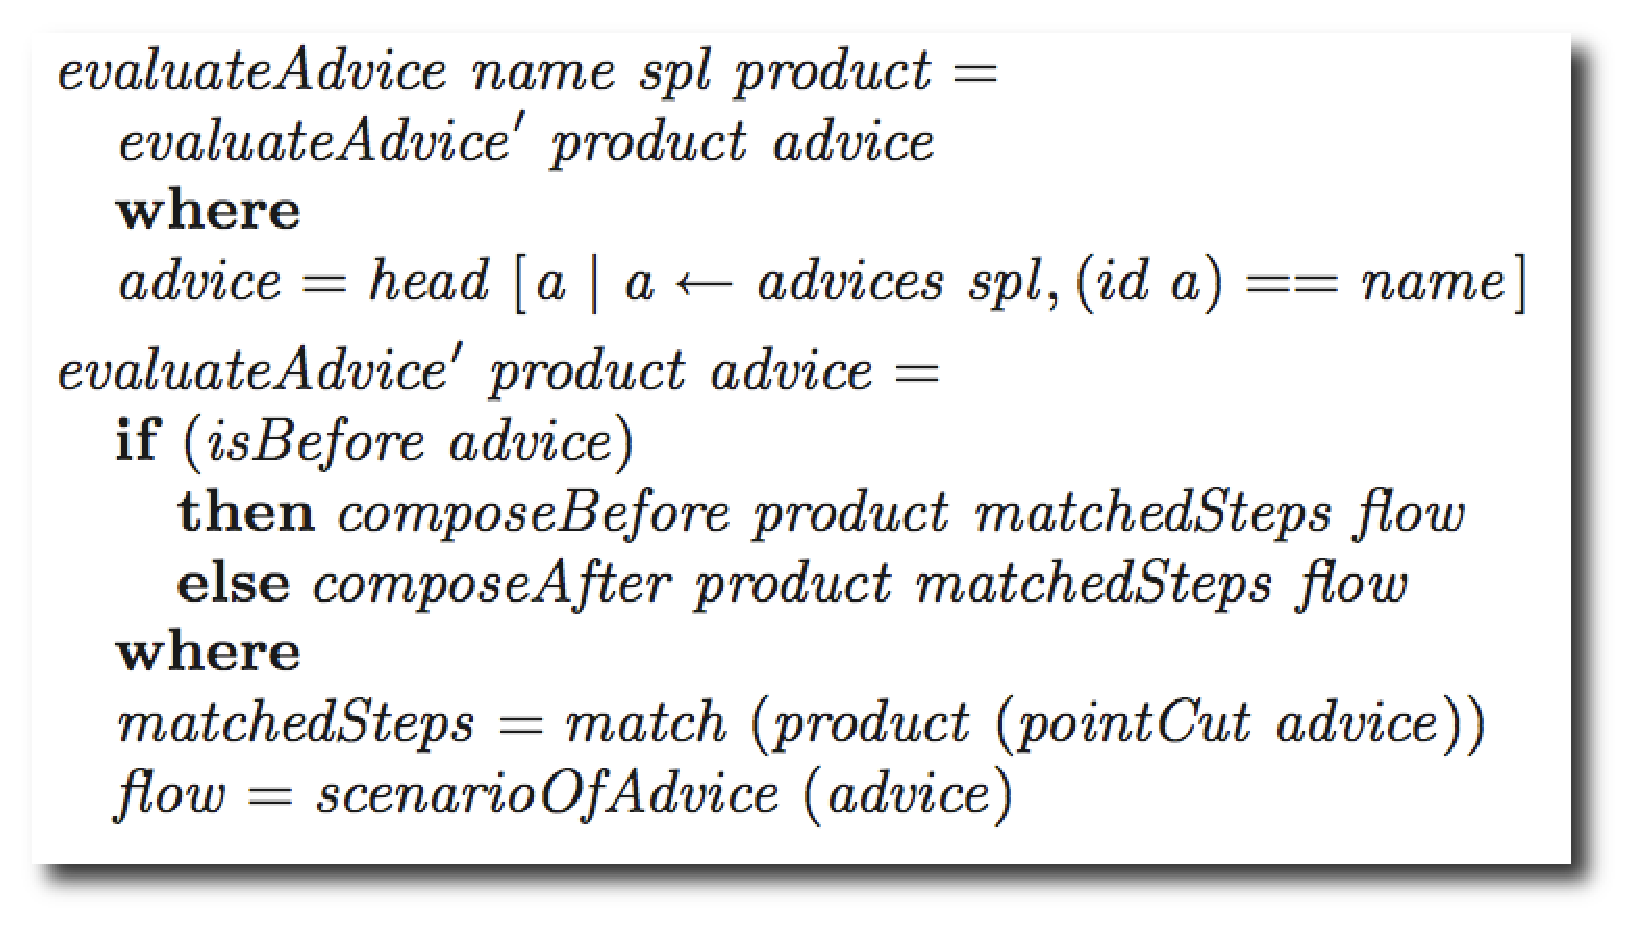
\includegraphics[scale=0.35]{img/evaluateAdviceReferenceImplementation.eps}
}
\end{center}
\end{block}
\end{frame}

\begin{frame}
\frametitle{Variability in Control Flow}
\begin{block}{Evaluate Aspect representation}

\begin{center} 
\center{
 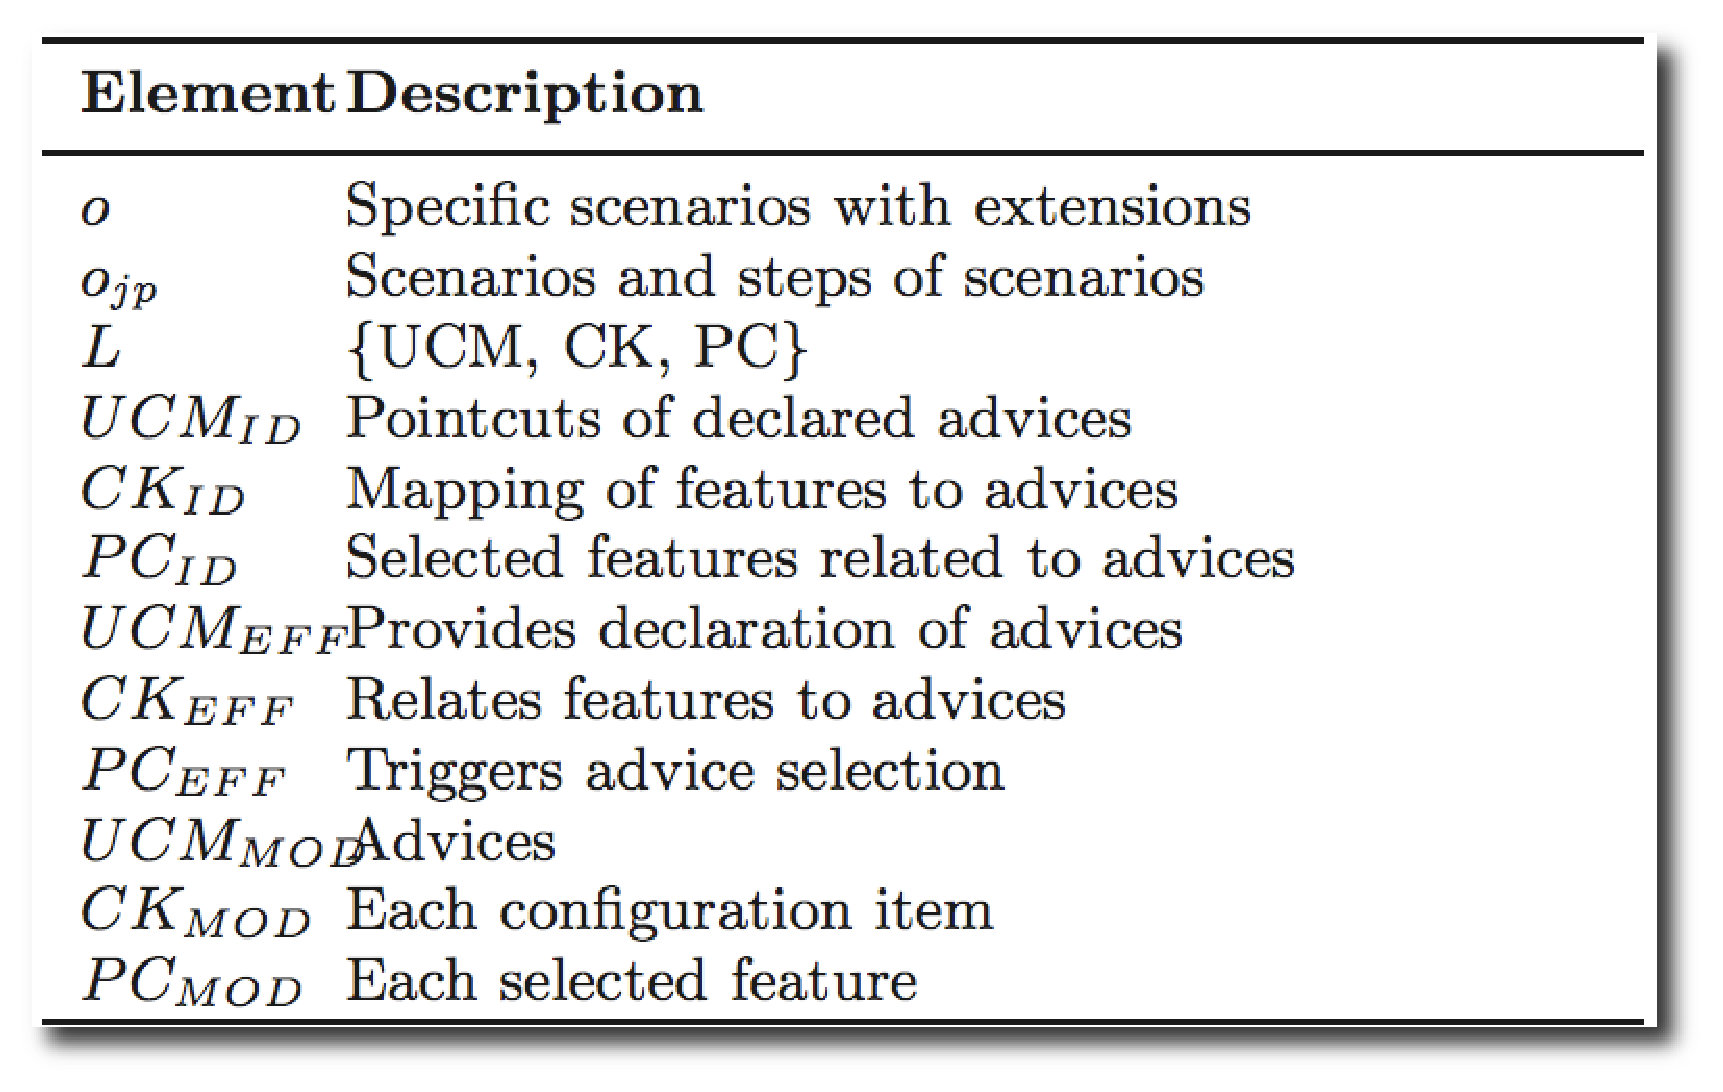
\includegraphics[scale=0.30]{img/evaluateAdviceModel.eps}
}
\end{center}

\end{block}
\end{frame}



\section{Evaluation}

\begin{frame}
\frametitle{Hypothesis}

\begin{block}{Our approah:}

\begin{itemize}
  \item H1. Improves both feature scattering and scenario cohesion
  \item H2. Reduces the time required to evolve SPLs
  \item H3. Adheres to the \emph{open-close} principle
\end{itemize}
\end{block}

\onslide+<2>

\begin{block}{Possible ``side effects'':}

\begin{itemize}
  \item H4. Might require more time to build the SPL specifications
  \item New challenge: interactions between advices might occur
\end{itemize}
\end{block}

\end{frame}

\begin{frame}
\frametitle{First Evaluation}

\begin{block}{Metrics}
\begin{itemize}
  \item Degree of Scattering 
  \item Degree of Focus
\end{itemize}
\end{block}

\begin{block}{Different case studies (low level of control):}
\begin{itemize}
  \item \emph{eCommerce}
  \item Smart Home
  \item Pedagogical Product Line
\end{itemize}
\end{block}

\end{frame}

\begin{frame}
\frametitle{First Evaluation}

\begin{block}{Findings}

Evidences about improvements on feature scattering and scenario
cohesion (H1). However, the results depend on several factors, such as:

\begin{itemize}
  \item Homogeneous x Heterogenous crosscutting 
  \item Number of alternative and optional features
\end{itemize} 
\end{block}

\end{frame}

\begin{frame}

\frametitle{Second Evaluation}

\begin{block}{Controlled experiment}
\begin{itemize}
\item Goal: restructure product specifications into SPL specification
\item Factors: students and product line domain
\item Treatments: PLUSS x SVCM
\item Response variable: time required to restructure the input specifications  
\end{itemize}
\end{block}

\begin{block}{Findings}
The results reveal to us that our approach (SVCM) require more time to 
restructure individual product specifications into SPL specification (confirms H4).   
\end{block}
\end{frame}

\begin{frame}
\frametitle{Third Evaluation}

\begin{block}{Controlled experiment}
\begin{itemize}
\item Goal: evolve SPL specifications according to a set of CRs
\item Factors: students and the sets of CRs
\item Treatments: PLUSS x SVCM
\item Response variables: 
\begin{itemize}
\item Feature scattering and scenario cohesion (H1)
\item Time required to evolve the SPLs (H2)
\item Degree of the \emph{open-close} principle (H3) %: $additions/(additions+changes)$
\end{itemize}
\end{itemize}

\end{block}

The results confirm both H1 and H3. However, they are inconclusive about H2.

\end{frame}


\section{Concluding remarks}

\begin{frame}
\frametitle{Concluding Remarks and Future Work}
\begin{block}{Research contributions}
\begin{itemize}
  \item Modular support for VM in use case scenarios
  \item A novel approach for representing VM 
  \item A suite of metrics and an evaluation process to our context 
\end{itemize}
\end{block}

\onslide+<2>

\begin{block}{Engineering contribution}
 \begin{itemize}
  \item A Haskell DSL for variability management
  \begin{itemize}
    \item Feature modeling 
    \item Product generation
  \end{itemize} 
\end{itemize}
\end{block}

\end{frame}

\begin{frame}
\frametitle{Concluding Remarks and Future Work}
\begin{block}{Next steps}
\begin{itemize}
  \item Plan and execute new experiments to verify our hypothesis
  \item Investigate the interaction problem between advices 
  \item Release a version of our Haskell libraries and tools
\end{itemize}
\end{block}

\end{frame}


\begin{frame}
\titlepage
\end{frame}

\end{document}
